\documentclass[letterpaper,11pt]{article}
\usepackage[empty]{fullpage}  % full page margin
\usepackage{baskervillef}  % Baskerville font
\usepackage[T1]{fontenc}  % font encoding
\usepackage[english]{babel}  % language
\usepackage{titlesec}  % custom section fonts
\usepackage{fancyhdr}  % header and footer
\usepackage[usenames,dvipsnames]{xcolor}  % colors
\usepackage{enumitem}  % list spacing
\usepackage[hidelinks]{hyperref}  % links
\usepackage{graphicx}  % images
\usepackage{tabularx}  % advanced tables
\usepackage{multicol}  % multiple columns

% --- typeset settings ---
% page layout
\pagestyle{fancy}
\fancyhf{} 
\fancyfoot{}
\setlength{\footskip}{10pt}
\renewcommand{\headrulewidth}{0pt}
\renewcommand{\footrulewidth}{0pt}

\addtolength{\oddsidemargin}{0.0in}
\addtolength{\evensidemargin}{0.0in}
\addtolength{\textwidth}{0.0in}
\addtolength{\topmargin}{0.2in}
\addtolength{\textheight}{0.0in}

% section format
\titleformat{\section}{
    \vspace{-15pt}
    \large\vspace{3pt}\scshape
}{}{0em}{}[\color{black}\titlerule]%\vspace{-5pt}]

% others
\urlstyle{same}  % url style
\raggedright  % left align
\setlength{\tabcolsep}{0in}  % table padding
\pdfgentounicode=1  % enable the generation of Unicode mappings in the PDF output

% --- custom commands ---
% resume listing
\newcommand{\resumeListingStart}{\begin{itemize}[leftmargin=0.15in, label={}]}
\newcommand{\resumeListingEnd}{\end{itemize}\vskip5pt}

\newcommand{\resumeEntry}[4]{
    % 2x2 standard entry in resume listing
    % the first 2 arguments are used for the main line
    % the last 2 arguments are used for the subline
    \vspace{-2pt}\item
        \begin{tabular*}{0.97\textwidth}[t]{l@{\extracolsep{\fill}}r}
            \textbf{#1} & #2 \\
            \textit{\small #3} & \textit{\small #4} \\
        \end{tabular*}\vspace{-10pt}
}

\newcommand{\resumeSubline}[1]{
    % additional subline in resume
    \vspace{-5pt}\item
        \begin{tabular*}{0.97\textwidth}[t]{l@{\extracolsep{\fill}}r}
            \textit{\small #1} &  \\
        \end{tabular*}\vspace{-17pt}
}

% resume itemize
\newenvironment{resumeItemize}
  {\begin{itemize}[leftmargin=0.15in, label={}, itemsep=0em]}
  {\end{itemize}}

% link with parentheses
\newcommand{\paralink}[2]{\href{#1}{\textsl{(#2)}}}

% bibliography
\usepackage[style=ieee, backend=biber, sorting=ydnt]{biblatex}
\DeclareFieldFormat{labelnumberwidth}{}
\setlength{\biblabelsep}{0pt}
\addbibresource{publications.bib}

\begin{document}
    \begin{center}
        % name
        {\LARGE Qi-Long Liu}\\
        
        % email
        \vskip5pt
        \url{qilong-kirov.liu@connect.polyu.hk}\\
        \vskip5pt
        
        % links
        \href
            {https://scholar.google.com/citations?user=N2-7ArsAAAAJ&hl=en}
            {Google Scholar 
\includegraphics[height=0.3cm]{icon/google-scholar.png}}
        \href
            {https://orcid.org/0000-0001-7843-1925}
            {ORCID 
\includegraphics[height=0.3cm]{icon/orcid.png}}
        \href
            {https://github.com/liu-qilong}
            {GitHub 
\includegraphics[height=0.3cm]{icon/github.png}}
        \href
            {https://qilong-liu.vercel.app}
            {Homepage 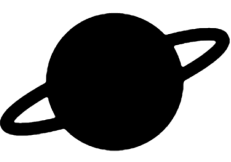
\includegraphics[height=0.3cm]{icon/blog.png}}
    \end{center}

    % education
    \section{Education}

    \resumeSubHeadingListStart
        \resumeSubheading
            {The Hong Kong Polytechnic University}{Sep 2021 -- Feb 2024}
            {Master of Philosophy, \href{https://www.aidlab.hk/en/}{Laboratory for Artificial Intelligence in Design (AiDLab)}}{Hong Kong, China}
            \resumeSubline{Supervised by \href{https://research.polyu.edu.hk/en/persons/kit-lun-yick}{Prof. Kit-lun Yick}, \href{https://www.polyu.edu.hk/en/pri/people/pri-people/dr-yip-yiu-wan-joanne/}{Prof. Joanne Yip} and Dr. Yue Sun}
        \resumeSubheading
            {Shenzhen University}{Sep 2017 -- Jul 2021}
            {Bachelor of Engineering, School of Biomedical Engineering}{Shenzhen, China}
            \resumeSubline{Supervised by \href{https://bme.szu.edu.cn/20161/0229/35.html}{Dr. Yongjin Zhou}}
    \resumeSubHeadingListEnd

    % awards
    \section{Awards}

    \resumeSubHeadingListStart
        \resumeSubheading
            {The Hong Kong Polytechnic University Research Studentship}{2021 -- 2023}
            {The Hong Kong Polytechnic University}{}
        \resumeSubheading
            {Star of Double Innovations (Group Award)}{2021}
            {Third Prize, Shenzhen University}{}
        \resumeSubheading
            {National College Students Biomedical Engineering Innovation Design Competition}{2019}
            {Third Prize, The Teaching Steering Committee of Biomedical Engineering in Colleges}{}
            \resumeSubline{and Universities of the Ministry of Education}
        \resumeSubheading
            {National College Students Electronic Design Competition in Guangdong Province}{2019}
            {Third Prize, The Organizing Committee of the Guangdong Province Division of }{}
            \resumeSubline{the National Undergraduate Electronic Design Competition}
    \resumeSubHeadingListEnd

    % publications
    \section{Publications}
    
    \begin{refsection}
        \begin{enumerate}[leftmargin=0.15in, label={}, itemsep=0em]
            \item \textbf{Under Review}
            \nocite{*}
            \printbibliography[keyword=review, heading=none]
            \item \textbf{Journal}
            \nocite{*}
            \printbibliography[type=article, notkeyword=review, heading=none]
            \newpage
            \item \textbf{Conference}
            \nocite{*}
            \printbibliography[type=inproceedings, notkeyword=review, heading=none]
            \item \textbf{Thesis}
            \nocite{*}
            \printbibliography[type=thesis, notkeyword=review, heading=none]
            \printbibliography[type=phdthesis, notkeyword=review, heading=none]
        \end{enumerate}
    \end{refsection}

    % work experience
    \section{Work \& research experience}

    \resumeSubHeadingListStart
        \resumeSubheading
            {The Hong Kong Polytechnic University}{Sep 2023 -- Present}
            {Research Assistant (full-time)}{Hong Kong, China}
            \resumeSubline{Supervised by \href{https://research.polyu.edu.hk/en/persons/kit-lun-yick}{Prof. Kit-lun Yick}}
            \resumeSubline{3D/4D scene reconstruction/understanding, dense motion tracking, and human pose analysis}
        \resumeSubheading
            {Shenzhen Base of The Hong Kong Polytechnic University}{Dec 2020 -- Jun 2021}
            {Student Assistant (part-time) for \href{https://research.polyu.edu.hk/en/persons/kit-lun-yick}{Prof. Kit-lun Yick}}{Shenzhen, Guangdong, China}
            \resumeSubline{Supervised by \href{https://research.polyu.edu.hk/en/persons/kit-lun-yick}{Prof. Kit-lun Yick}}
            \resumeSubline{3D/4D scanning data cleansing, labelling, and processing}
        \resumeSubheading
            {Shenzhen Zhishixinyun Educational Technology Ltd.}{Nov 2019 -- Mar 2020}
            {Python tutorial lecturer (internship)}{Shenzhen, Guangdong, China}
    \resumeSubHeadingListEnd

    % projects
    \section{Open-source projects \emph{(selected)}}

    \resumeSubHeadingListStart
        \resumeSubheading
            {PaperThread}{2023}
            {Visualize papers' relations as threads}{\href{https://github.com/liu-qilong/obsidian-setup}{\underline{Link}}}
        \resumeSubheading
            {FEcluster}{2023}
            {Distribute FE simulation tasks across multiple computers via SSH}{\href{https://github.com/liu-qilong/FEcluster}{\underline{Link}}}
        \resumeSubheading
            {mesh4d}{2023}
            {Toolkit for 4D (3D + T) data visualisation, operation, and dynamic estimation}{\href{https://github.com/liu-qilong/mesh4d}{\underline{Link}}}
        \resumeSubheading
            {qilong-liu.vercel.app}{2023}
            {Minimalist personal blog site based on Next.js and Tailwind}{\href{https://github.com/liu-qilong/qilong-liu}{\underline{Link}}}
        \resumeSubheading
            {pedarProbe}{2022}
            {Data analysis framework for pedar plantar pressure sensor}{\href{https://github.com/liu-qilong/pedarProbe}{\underline{Link}}}
        \resumeSubheading
            {Beamer-LaTeX-Themes}{2022}
            {Customized beamer templates for PolyU, SZU, and more}{\href{https://github.com/liu-qilong/Beamer-LaTeX-Themes}{\underline{Link}}}
    \resumeSubHeadingListEnd

    % skills
    \section{Skill set}

    \begin{itemize}[leftmargin=0.15in, label={}, itemsep=0em]
        \item \textbf{Languages}\\
        English (fluent); Mandarin (native); Cantonese (native)
        \item \textbf{Programming}\\
        Python (seasoned); JavaScript (intermediate); Bash shell scripting (intermediate); C/C++ (basic); Matlab (intermediate)
        \item \textbf{Others}\\
        LaTeX (seasoned); TikZ (intermediate); Git (seasoned); Docker (basic); Next.js (seasoned); Sphinx (seasoned)
    \end{itemize}

\end{document}
